\documentclass{standalone}
\usepackage{tikz}
%\usetikzlibrary{...}
\begin{document}
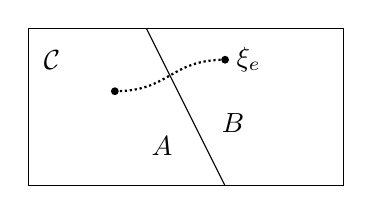
\begin{tikzpicture}
\draw (0,-2) rectangle (4,0);

\draw (2.5,-2) -- (1.5,0);

\node (clab) at (0.3,-0.4) {$\mathcal{C}$};



\draw[thick,densely dotted]
   (1.1,-0.8) .. controls (1.8,-0.8) and (1.8,-0.4) .. (2.5,-0.4);
   
\node[circle,fill=black,inner sep=1pt] at (1.1,-0.8) {};
\node[circle,fill=black,inner sep=1pt] at (2.5,-0.4) {};

\node at (1.7,-1.5) {$A$};
\node at (2.6,-1.2) {$B$};

\node at (2.8,-0.4) {$\xi_e$};

\end{tikzpicture}%
\end{document}
